\subsection{欧拉积分}

为简便起见，我们称一个函数 \(f\) （定义在区间 \(I \subset \mathbf{R}\) 上，且在此区间上 \(> 0\) ）在 \(I\) 上是对数凸的，如果 \(\log f\) 在 \(I\) 上是凸的。\(\Gamma(x)\) 的定义表明这个函数在 \(]0, +\infty[\) 上是对数凸的。

显然，I 上两个对数凸函数的乘积在 I 上也是对数凸的。此外：

引理 1. 设 \(f\) 与 \(g\) 是开区间 I 上两个 \(> 0\) 且两次可导的函数。若 \(f\) 与 \(g\) 都是 I 上的对数凸函数，则 \(f + g\) 在 I 上也是对数凸的。

关系式 \(\mathrm{D}^{2}\left(\log f(x)\right) \geqslant 0\) 可以写成 \(f(x)f''(x) - \left(f'(x)\right)^{2} \geqslant 0\) 。于是只需证明：关系式 a \textgreater{} 0、\(a' > 0\)、\(ac - b^{2} \geqslant 0\)、\(a'c' - b'^{2} \geqslant 0\) 蕴含 \((a + a')(c + c') - (b + b')^{2} \geqslant 0\) ；而当 a \textgreater{} 0 时，关系式 \(ac - b^{2} \geqslant 0\) 等价于二次型 \(ax^{2} + 2bxy + cy^{2}\) 为 \(\geqslant 0\) （在 \(R^{2}\) 上）这一事实，且显然，若

\[
a x ^ {2} + 2 b x y + c y ^ {2} \geqslant 0 \quad \text { and } \quad a ^ {\prime} x ^ {2} + 2 b ^ {\prime} x y + c ^ {\prime} y ^ {2} \geqslant 0
\]

在 \(\mathbf{R}^{2}\) 上成立，则 \((a + a')x^{2} + 2(b + b')xy + (c + c')y^{2} \geqslant 0\) 在 \(\mathbf{R}^{2}\) 上也成立。

引理 2. 设 \(f\) 是一个有限实值函数，\(>0\) ，在积 \(I \times J\) （\(\mathbf{R}\) 中两个开区间之积）上有定义且连续，并使得对每个 \(t \in J\) ，函数 \(x \mapsto f(x,t)\) 在 \(I\) 上是对数凸的且两次可导。在这些假设下，若积分 \(g(x) = \int_{J} f(x,t) dt\) 对每个 \(x \in I\) 收敛，则 \(g\) 在 \(I\) 上是对数凸的。

首先证明，对每个紧区间 \(K \subset J\) ，函数 \(g_{K}(x) = \int_{K} f(x, t) dt\) 是对数凸的。事实上，若 \(K = [a, b]\) ，则函数序列

\[
g _ {n} (x) = \frac {b - a}{n} \sum_ {k = 0} ^ {n - 1} f \left(x, a + k \frac {b - a}{n}\right)
\]

在 I 上简单收敛于 \(g_{K}(x)\) （II, p.~57, prop. 5），因而 \(\log g_{n}\) 简单收敛于 \(\log g_{K}\) ；由 VII, p.~310 的引理 1，\(\log g_{n}\) 在 I 上是凸的，故（I, p.~27, prop. 4）\(\log g_{K}\) 也是凸的。

另一方面，g 是 \(g_{K}\) 沿 I 的紧子区间所成的定向集的逐点极限（II, p.~64），故 \(\log g\) 是诸 \(\log g_{K}\) 的逐点极限；这些函数在 I 上都是凸的，因而 \(\log g\) 也是凸的（I, p.~27, prop. 4）。

容易证明，即使不假设函数两次可导，引理 1 与引理 2 仍然成立（VII, p.~327, exerc. 5）。

引理 3. 设 \(\varphi\) 是一个连续且 \(>0\) 的函数，定义在开区间 \(J\) （含于 \([0, +\infty[\) ）上。若 \(I\) 是使积分 \(g(x) = \int_{J} t^{x-1} \varphi(t) dt\) 对一切 \(x \in I\) 收敛的开区间，则 \(g\) 在 \(I\) 上是对数凸的。

事实上，\(\log t^{x - 1} = (x - 1)\log t\) 作为 \(x\) 的函数，对一切 \(t > 0\) 是凸的且两次可导的，故引理 2 适用。

命题 3. 对一切 \(x > 0\)

\[
\Gamma (x) = \int_ {0} ^ {\infty} e ^ {- t} t ^ {x - 1} d t\tag{14}
\]

（第二类欧拉积分）。

现在，函数 \(g(x) = \int_0^\infty e^{-t} t^{x-1} dt\) 对一切 \(x > 0\) 有定义（V, p.~229）；于是由 VII, p.~311 的引理 3，它在 \(]0, +\infty[\) 上是对数凸的。此外，分部积分给出

\[
g (x + 1) = \int_ {0} ^ {\infty} e ^ {- t} t ^ {x} d t = - e ^ {- t} t ^ {x} \Big | _ {0} ^ {\infty} + x \int_ {0} ^ {\infty} e ^ {- t} t ^ {x - 1} d t = x g (x).
\]

换句话说，g 是 VII, p.~305 的方程 (1) 的一个解；最后，

\[
g (1) = \int_ {0} ^ {\infty} e ^ {- t} d t = 1;
\]

因而命题由 VII, p.~306 的 prop. 1 得出。

由变量替换 \(e^{-t}=u\) ，从 (14) （VII, p.~311）推出公式

\[
\Gamma (x) = \int_ {0} ^ {1} \left(\log \frac {1}{t}\right) ^ {x - 1} d t.\tag{15}
\]

同样，由变量替换 \(u = t^{x}\) 得到

\[
x \Gamma (x) = \int_ {0} ^ {\infty} e ^ {- t ^ {1 / x}} d t
\]

或者再利用 (7) （VII, p.~3），得

\[
\Gamma \left(1 + \frac {1}{x}\right) = \int_ {0} ^ {\infty} e ^ {- t ^ {x}} d t\tag{16}
\]

而特别地，对 \(x = 2\) ，有

\[
\Gamma \left(\frac {3}{2}\right) = \frac {1}{2} \Gamma \left(\frac {1}{2}\right) = \int_ {0} ^ {\infty} e ^ {- t ^ {2}} d t.\tag{17}
\]

命题 4. 对 x \textgreater{} 0 与 y \textgreater{} 0 ，积分

\[
\mathbf {B} (x, y) = \int_ {0} ^ {1} t ^ {x - 1} (1 - y) ^ {y - 1} d t
\]

（第一类欧拉积分）取值

\[
\mathbf {B} (x, y) = \frac {\Gamma (x) \Gamma (y)}{\Gamma (x + y)}.\tag{18}
\]

事实上，这个积分对 \(x > 0\) 与 \(y > 0\) 收敛（V, p.~229）。由 VII, p.~311 的引理 3，函数 \(x \mapsto \mathbf{B}(x, y)\) 对 \(x > 0\) 是对数凸的。此外，

\[
\mathbf {B} (x + 1, y) = \int_ {0} ^ {1} (1 - t) ^ {x + y - 1} \left(\frac {t}{1 - t}\right) ^ {x} d t
\]

于是，由分部积分得

\[
\begin{array}{l} \mathbf {B} (x + 1, y) = - \frac {(1 - t) ^ {x + y}}{x + y} \left(\frac {t}{1 - t}\right) ^ {x} \Bigg | _ {0} ^ {1} \\ \qquad + \frac {x}{x + y} \int_ {0} ^ {1} (1 - t) ^ {x + y} \left(\frac {t}{1 - t}\right) ^ {x - 1} \frac {d t}{(1 - t) ^ {2}} = \frac {x}{x + y} \mathbf {B} (x, y). \end{array}
\]

由此推出，\(f(x) = \mathbf{B}(x, y) \Gamma(x + y)\) 满足 VII, p.~305 的恒等式 (1) 。而且，这个函数作为两个对数凸函数的乘积，是对数凸的。最后，有 \(f(1) = \mathbf{B}(1, y) \Gamma(y + 1)\) ，而 \(\mathbf{B}(1, y) = \int_{0}^{1} (1 - t)^{y - 1} dt = 1/y\) ，故 \(f(1) = \frac{1}{y} \Gamma(y + 1) = \Gamma(y)\) 。于是由 VII, p.~306 的 prop. 1，函数 \(f(x)/\Gamma(y)\) 等于 \(\Gamma(x)\) ，这就证明了 (18)。

由变量替换 \(t = \frac{u}{u + 1}\) ，公式 (18) 变为

\[
\int_ {0} ^ {\infty} \frac {t ^ {x - 1}}{(1 + t) ^ {x + y}} d t = \frac {\Gamma (x) \Gamma (y)}{\Gamma (x + y)}\tag{19}
\]

而由变量替换 \(t = \sin^{2} \varphi\) ，得

\[
\int_ {0} ^ {\pi / 2} \sin^ {2 x - 1} \varphi \cos^ {2 y - 1} \varphi d \varphi = \frac {1}{2} \frac {\Gamma (x) \Gamma (y)}{\Gamma (x + y)}.\tag{20}
\]

在这最后一个公式中取 \(x = y = \frac{1}{2}\) ，便得

\[
\Gamma (\frac {1}{2}) = \sqrt {\pi}\tag{21}
\]

再由 (17) ，得

\[
\int_ {0} ^ {\infty} e ^ {- t ^ {2}} d t = \frac {1}{2} \sqrt {\pi}.\tag{22}
\]

由 VII, p.~307 的关系式 (7) ，有渐近展开

\[
\begin{array}{l} \Gamma (x) = \frac {1}{x} \Gamma (x + 1) \\ = \frac {1}{x} + \Gamma^ {\prime} (1) + \frac {1}{2 !} \Gamma^ {\prime \prime} (1) x + \dots + \frac {1}{n !} \Gamma^ {(n)} (1) x ^ {n - 1} + O (x ^ {n}) \end{array}\tag{23}
\]

这是 \(\Gamma(x)\) 在 0 的一个邻域中的渐近展开。

同样，对每个固定的 y 且 \textgreater{} 0 ，可以写出

\[
\begin{array}{l} \frac {1}{\Gamma (x + y)} = \frac {1}{\Gamma (y)} + D \left(\frac {1}{\Gamma (y)}\right) x \\ \qquad + \frac {1}{2 !} D ^ {2} \left(\frac {1}{\Gamma (y)}\right) x ^ {2} + \dots + \frac {1}{n !} D ^ {n} \left(\frac {1}{\Gamma (y)}\right) x ^ {n} + O _ {1} (x ^ {n + 1}) \end{array}
\]

于是公式 (18) 给出，对固定的 y ，渐近展开

\[
\begin{array}{l} \mathbf {B} (x, y) = \frac {1}{x} + \left(\Gamma^ {\prime} (1) - \frac {\Gamma^ {\prime} (y)}{\Gamma (y)}\right) \\ \qquad + \left(\frac {\Gamma^ {\prime \prime} (1)}{2} - \Gamma^ {\prime} (1) \frac {\Gamma^ {\prime} (y)}{\Gamma (y)} + \frac {2 \Gamma^ {\prime 2} (y) - \Gamma (y) \Gamma^ {\prime \prime} (y)}{2 \Gamma^ {2} (y)}\right) x + O (x ^ {2}) \end{array}\tag{24}
\]

在 \(x = 0\) 的一个邻域中成立。

此外，对 x \textgreater{} 0 与 y \textgreater{} 0 ，有

\[
\begin{array}{l} \mathbf {B} (x, y) = \int_ {0} ^ {1} \left(t ^ {x - 1} + t ^ {x} \frac {(1 - t) ^ {y - 1} - 1}{t}\right) d t \\ = \frac {1}{x} + \int_ {0} ^ {1} t ^ {x} \frac {(1 - t) ^ {y - 1} - 1}{t} d t. \end{array}\tag{25}
\]

函数 \(\varphi(t) = \frac{(1 - t)^{y - 1} - 1}{t}\) 在紧区间 {[}0, 1{]} 上连续；由于

\[
t ^ {x} = e ^ {x \log t} = 1 + x \log t + \frac {x ^ {2}}{2 !} (\log t) ^ {2} + \dots + \frac {x ^ {n}}{n !} (\log t) ^ {n} + r _ {n} (x, t)
\]

其中 \(|r_n(x,t)| \leqslant \frac{x^{n+1}}{(n+1)!} |\log t|^{n+1}\) （因为 \(\log t \leqslant 0\) 且 \(x > 0\) ），公式 (25) 给出渐近展开

\[
\begin{array}{l} \mathbf {B} (x, y) = \frac {1}{x} + \int_ {0} ^ {1} \varphi (t) d t + x \int_ {0} ^ {1} \varphi (t) \log t d t + \dots \\ \qquad + \frac {x ^ {n}}{n !} \int_ {0} ^ {1} \varphi (t) (\log t) ^ {n} d t + O _ {2} (x ^ {n + 1}) \end{array}
\]

这是 \(\mathbf{B}(x,y)\) 在 0 的一个邻域中的渐近展开。

对 \(n = 1\) ，把这一展开与 (24) 等同起来，特别得到

\[
\Gamma^ {\prime} (1) - \frac {\Gamma^ {\prime} (y)}{\Gamma (y)} = \int_ {0} ^ {1} \frac {(1 - t) ^ {y - 1} - 1}{t} d t.
\]

此外，公式 (10) 给出 \(\Gamma'(1) = \Gamma'(1)/\Gamma(1) = -\gamma\) ，于是（高斯积分）

\[
\frac {\Gamma^ {\prime} (x)}{\Gamma (x)} + \gamma = \int_ {0} ^ {1} \frac {1 - (1 - t) ^ {x - 1}}{t} d t.\tag{26}
\]

\section{复数域中的 Γ 函数}

\subsection{Γ 函数到 C 上的延拓}

我们回到魏尔斯特拉斯公式，它给出表达式

\[
\frac {1}{\Gamma (x)} = x e ^ {\gamma x} \prod_ {n = 1} ^ {\infty} \left(1 + \frac {x}{n}\right) e ^ {- x / n}\tag{1}
\]

\(1 / \Gamma (x)\) （对一切实数 \(x\) ）；现考虑以 \(\left(1 + \frac{z}{n}\right)e^{-z / n}\) 为通项、以任意复数 \(z\) 为变量的无穷乘积。可以写 \(e^{-z / n} = 1 - \frac{z}{n} + h(z)\) ，其中 \(|h(z)| \leqslant \frac{|z|^2}{2n^2} e^{|z / n|}\) （III, p.~106, 公式 (8)），于是

\[
\left(1 + \frac {z}{n}\right) e ^ {- z / n} = 1 + v _ {n} (z)
\]

其中 \(|v_{n}(z)| \leqslant \frac{|z|^{2}}{n^{2}}\left(1 + \frac{e^{|z|}}{2}(1 + |z|)\right)\) ；因此所考虑的无穷乘积在 C 的每个紧子集上绝对且一致收敛；而且，它的值仅在点 z = -n 处为零（Gen.~Top., IX, p.~214, corollary）。鉴于 VII, p.~315 的公式 (1) ，对每个复数 z ，令

\[
\frac {1}{\Gamma (z)} = z e ^ {\gamma z} \prod_ {n = 1} ^ {\infty} \left(1 + \frac {z}{n}\right) e ^ {- z / n}.\tag{2}
\]

这样，函数 \(\Gamma(z)\) 对每个点 \(z \in \mathbf{C}\) （除点 \(-n\) （ \(n \in \mathbf{N}\) ）以外）都有定义；它在这个集合上连续，并且 \((z + n)\Gamma(z) \sim \frac{(-1)^n}{n!}\) （在 \(-n\) 的一个邻域中）。公式 (2) 表明，有 \(\Gamma(\overline{z}) = \overline{\Gamma(z)}\) （对每个异于负整数的 \(z\) ）。

从高斯公式（VII, p.~307, 公式 (8)）过渡到魏尔斯特拉斯公式的论证，将其中的步骤倒转，也适用于复数 \(z\) ，并且表明，对 \(z \neq -n\) （ \(n \in \mathbf{N}\) ），有

\[
\Gamma (z) = \lim _ {n \rightarrow \infty} \frac {n ^ {z} n !}{z (z + 1) \dots (z + n)}\tag{3}
\]

这里约定取 \(n^z = e^{z\log n}\) 。由于

\[
\frac {n ^ {z + 1} n !}{(z + 1) (z + 2) \dots (z + n + 1)} = z \frac {n}{n + 1 + z} \frac {n ^ {z} n !}{z (z + 1) \dots (z + n)}
\]

取极限，再次得到基本泛函方程

\[
\Gamma (z + 1) = z \Gamma (z)\tag{4}
\]

对每个 \(z \neq -n (n \in \mathbf{N})\) 成立。

设 \(p\) 是任意整数 \(> 0\) ，\(\mathrm{K}_p\) 为开圆盘 \(|z| < p\) ；对每个 \(z \in \mathrm{K}_p\) 与每个整数 \(n > p\) ，\(1 + \frac{z}{n}\) 不是负实数，故 \(\log \left(1 + \frac{z}{n}\right)\) 有定义，且由上所述，以 \(\log \left(1 + \frac{z}{n}\right) - \frac{z}{n} (n > p)\) 为通项的级数在 \(\mathrm{K}_p\) 上正规收敛；对通项微分有限次所得的级数也同样如此，因为有

\[
\left| \frac {1}{n} - \frac {1}{z + n} \right| \leqslant \frac {p}{n (n - p)} \quad \text { and } \quad \left| \frac {1}{(z + n) ^ {k}} \right| \leqslant \frac {1}{(n - p) ^ {k}} \quad (k > 1)
\]

对 \(z \in \mathbf{K}_p\) 与 \(n > p\) 成立。于是可以看出（cf.~II, p.~59, 注 3），\(\Gamma(z)\) 在所有点 \(z \in \mathbf{C}\) （除诸点 \(-n\) 以外）处无穷次可导，且在这些点处有

\[
{\frac {\Gamma^ {\prime} (z)}{\Gamma (z)}} = - \gamma - {\frac {1}{z}} + \sum_ {n = 1} ^ {\infty} \left({\frac {1}{n}} - {\frac {1}{z + n}}\right)\tag{5}
\]

\[
\mathrm{D} ^ {k - 1} \left(\frac {\Gamma^ {\prime} (z)}{\Gamma (z)}\right) = \sum_ {n = 0} ^ {\infty} \frac {(- 1) ^ {k} (k - 1) !}{(z + n) ^ {k}} \quad \text { for } \quad k \geqslant 2,\tag{6}
\]

其中 (5) 与 (6) 的右端在 \(\mathbf{C}\) 的每个不含任何整数 \(\leqslant 0\) 的紧子集上正规收敛。此外，可以写

\[
\log \Gamma (z) \equiv - \gamma z - \log z + \sum_ {n = 1} ^ {\infty} \left(\frac {z}{n} - \log \left(1 + \frac {z}{n}\right)\right) \pmod {2 \pi i}\tag{7}
\]

这里约定：当此公式中的某个对数是负实数的对数时，就在该点处取相差 \(2\pi i\) 的 \(\log z\) 的这一个或那一个极限值；于是 (7) 右端的级数在 C 的每个不含任何整数 \(\leqslant 0\) 的紧子集上正规收敛。

\subsection{余元公式与勒让德–高斯倍乘公式}

由 VII, p.~315 的公式 (2) 立即导出，对每个 \(z \in C\) ，

\[
\frac {1}{\Gamma (z) \Gamma (- z)} = - z ^ {2} \prod_ {n = 1} ^ {\infty} \left(1 - \frac {z ^ {2}}{n ^ {2}}\right).
\]

而 \(\sin z\) 的欧拉展开（VI, p.~287, th. 2）表明

\[
z \prod_ {n = 1} ^ {\infty} \left(1 - \frac {z ^ {2}}{n ^ {2}}\right) = \frac {1}{\pi} \sin \pi z;
\]

再利用 VII, p.~315 的泛函方程 (4) ，便得到：

命题 1. 对每个复数 \(z\) ，有

\[
\frac {1}{\Gamma (z) \Gamma (1 - z)} = \frac {1}{\pi} \sin \pi z\tag{8}
\]

（余元公式）。

推论 --- 对每个实数 t ，有

\[
| \Gamma (i t) | = \sqrt {\frac {\pi}{t \sinh \pi t}} \qquad (t \neq 0)\tag{9}
\]

\[
\left| \Gamma (\frac {1}{2} + i t) \right| = \sqrt {\frac {\pi}{\cosh \pi t}}.\tag{10}
\]

事实上，由 (8) 推出 \(\Gamma(it)\Gamma(-it) = \frac{i\pi}{t\sin\pi it} = \frac{\pi}{t\sinh\pi t}\) ，且有 \(\Gamma(-it) = \overline{\Gamma(it)}\) ；同样，(8) 给出

\[
\Gamma \left(\frac {1}{2} + i t\right) \Gamma \left(\frac {1}{2} - i t\right) = \frac {\pi}{\sin \left(\frac {\pi}{2} + \pi i t\right)} = \frac {\pi}{\cos \pi i t} = \frac {\pi}{\cosh \pi t},
\]

并且有

\[
\Gamma \bigl (\frac {1}{2} - i t \bigr) = \overline {{\Gamma \bigl (\frac {1}{2} + i t \bigr)}}.
\]

现设 \(p\) 是任意整数 \(> 0\) ，考虑乘积

\[
f (z) = \Gamma \left(\frac {z + 1}{p}\right) \Gamma \left(\frac {z + 2}{p}\right) \dots \Gamma \left(\frac {z + p}{p}\right).
\]

由 (3) （VII, p.~315），对每个 \(z \neq -n\) （ \(n \in \mathbf{N}\) ），\(f(z)\) 是乘积

\[
\begin{array}{c} \frac {n ^ {(z + 1) / p} n !}{\left(\frac {z + 1}{p}\right) \left(\frac {z + 1}{p} + 1\right) \cdots \left(\frac {z + 1}{p} + n\right)}. \\ \frac {n ^ {(z + 2) / p} n !}{\left(\frac {z + 2}{p}\right) \left(\frac {z + 2}{p} + 1\right) \cdots \left(\frac {z + 2}{p} + n\right)} \dots \\ \dots \frac {n ^ {(z + p) / p} n !}{\left(\frac {z + p}{p}\right) \left(\frac {z + p}{p} + 1\right) \cdots \left(\frac {z + p}{p} + n\right)} \\ = \frac {n ^ {z + (p + 1) / 2} p ^ {(n + 1) p} (n !) ^ {p}}{(z + 1) (z + 2) \ldots (z + (n + 1) p)} \end{array}
\]

的极限；特别地，\(f(0)\) 是乘积

\[
\frac {n ^ {(p + 1) / 2} p ^ {(n + 1) p} (n !) ^ {p}}{((n + 1) p) !}
\]

由此推出，\(f(z) / f(0)\) 是

\[
\begin{array}{c} \frac {n ^ {z} ((n + 1) p) !}{(z + 1) (z + 2) \dots (z + (n + 1) p)} \\ = z   p ^ {- z} \left(\frac {n}{n + 1}\right) ^ {z}. \frac {((n + 1) p) ^ {z} ((n + 1) p) !}{z (z + 1) (z + 2) \dots (z + (n + 1) p)} \end{array}
\]

的极限；于是由 (3) （VII, p.~315）得

\[
f (z) = f (0) z p ^ {- z} \Gamma (z).\tag{11}
\]

但是，可以写

\[
f (0) = \prod_ {k = 1} ^ {p - 1} \Gamma \left(\frac {k}{p}\right) = \prod_ {k = 1} ^ {p - 1} \Gamma \left(1 - \frac {k}{p}\right) = \sqrt {\prod_ {k = 1} ^ {p - 1} \Gamma \left(\frac {k}{p}\right) \Gamma \left(1 - \frac {k}{p}\right)}
\]

由于 \(f(0) > 0\) ；于是余元公式给出

\[
f (0) = \sqrt {\pi^ {p - 1} / \prod_ {k = 1} ^ {p - 1} \sin \frac {k \pi}{p}}
\]

又由于右端的乘积等于 \(p/2^{p-1}\) （VI, p.~284, cor. 1），最终得到：

命题 2. 对每个不是整数 \(\leqslant 0\) 的复数 z 以及每个整数 p \textgreater{} 0 ，有

\[
\Gamma \left(\frac {z}{p}\right) \Gamma \left(\frac {z + 1}{p}\right) \dots \Gamma \left(\frac {z + p - 1}{p}\right) = (2 \pi) ^ {(p - 1) / 2} p ^ {\frac {1}{2} - z} \Gamma (z)\tag{12}
\]

（勒让德–高斯倍乘公式）。

命题 3. 对每个实数 x \textgreater{} 0 ，有

\[
\int_ {x} ^ {x + 1} \log \Gamma (t) d t = x (\log x - 1) + \frac {1}{2} \log 2 \pi\tag{13}
\]

（拉阿贝积分）。

首先对 \(x = 0\) 证明公式 (13) 。由于 \(\log \Gamma(x) \sim \log \frac{1}{x}\) （当 \(x\) 趋于 0 时），积分 \(\int_0^1 \log \Gamma(x) dx\) 收敛。此外，函数 \(\log \Gamma(x)\) 在 {[}0, 1{]} 上递减（VII, p.~310）；于是对每个 \(\alpha > 0\) 有

\[
\frac {1}{n} \sum_ {k = 1} ^ {q} \log \Gamma \left(\frac {k}{n}\right) \leqslant \int_ {0} ^ {\alpha} \log \Gamma (x) d x,
\]

其中 \(q\) 是使 \(q / n \leqslant \alpha\) 的最大整数。由于 \(\int_{0}^{\alpha} \log \Gamma(x) dx\) 随 \(\alpha\) 而趋于 0 ，且 \(\frac{1}{n} \sum_{k=q+1}^{n} \log \Gamma\left(\frac{k}{n}\right)\) 趋于 \(\int_{\alpha}^{1} \log \Gamma(x) dx\) （当 \(n\) 趋于 \(+\infty\) 时；II, p.~57, prop. 5） ，故有

\[
\int_ {0} ^ {1} \log \Gamma (x) d x = \lim _ {n \rightarrow \infty} \frac {1}{n} \sum_ {k = 1} ^ {n} \log \Gamma \left(\frac {k}{n}\right).
\]

而由 (12) ，此公式右端是

\[
\frac {n - 1}{2 n} \log 2 \pi - \frac {1}{2} \frac {\log n}{n},
\]

的极限，由此得

\[
\int_ {0} ^ {1} \log \Gamma (x) d x = \frac {1}{2} \log 2 \pi .\tag{14}
\]

其次我们注意到，由恒等式

\[
\log \Gamma (x + 1) = \log \Gamma (x) + \log x
\]

积分后得到，对 x \textgreater{} 0

\[
\int_ {0} ^ {x} \log \Gamma (t + 1) d t = \int_ {0} ^ {x} \log \Gamma (t) d t + \int_ {0} ^ {x} \log t d t.
\]

但左端的积分也等于 \(\int_{1}^{x + 1}\log \Gamma (t)dt\) 。于是由 (14) ，

\[
\int_ {x} ^ {x + 1} \log \Gamma (t) d t = \int_ {0} ^ {x} \log t d t + \frac {1}{2} \log 2 \pi = x (\log x - 1) + \frac {1}{2} \log 2 \pi .
\]

\subsection{斯特林展开}

设 \(x\) 与 \(y\) 是两个不在实负半轴上的复数；由 VII, p.~315 的公式 (3) ，并依照 VII, p.~316 关于对数的约定，\(\log \Gamma(x) - \log \Gamma(y)\) 模 \(2\pi i\) 同余于表达式

\[
(x - y) \log n + \sum_ {k = 0} ^ {n} \Big (\log (y + k) - \log (x + k) \Big).\tag{15}
\]

令 \(f(t) = \log(y + t) - \log(x + t)\) ；对函数 f 应用欧拉–麦克劳林求和公式（VI, p.~288）：

\[
\begin{array}{l} f (0) + f (1) + \dots + f (n) = \int_ {0} ^ {n + 1} f (t) d t - \frac {1}{2} \big (f (n + 1) - f (0) \big) \\ \qquad + \sum_ {k = 1} ^ {p} \frac {b _ {2 k}}{(2 k) !} \big (f ^ {(2 k - 1)} (n + 1) - f ^ {(2 k - 1)} (0) \big) + T _ {p} (n) \end{array}
\]

其中

\[
\left| \mathrm{T} _ {p} (n) \right| \leqslant \frac {4 e ^ {2 \pi}}{(2 \pi) ^ {2 p + 1}} \int_ {0} ^ {n + 1} \left| f ^ {(2 p + 1)} (u) \right| d u.\tag{16}
\]

由于

\[
f ^ {(m)} (t) = (- 1) ^ {m - 1} (m - 1)! \left(\frac {1}{(y + t) ^ {m}} - \frac {1}{(x + t) ^ {m}}\right),
\]

\(f^{(2k - 1)}(n + 1)\) 当 \(n\) 趋于 \(+\infty\) 时趋于 0 （对一切 \(k \geqslant 1\) ）；对

\[
f (n + 1) = \log \left(1 + \frac {y}{n + 1}\right) - \log \left(1 + \frac {x}{n + 1}\right).
\]

此外，有

\[
\int_ {0} ^ {n + 1} \log (x + t) d t = (x + n + 1) (\log (x + n + 1) - 1) - x (\log x - 1);
\]

当 n 趋于 \(+\infty\) 时，有渐近展开

\[
(x + n) \bigl (\log (x + n) - 1 \bigr) = n \log n - n + x \log n + O \left(\frac {1}{n}\right).
\]

把这些结果代入表达式 (15) ，最终可以看出，当 n 趋于 \(+\infty\) 时，\(\mathrm{T}_{p}(n)\) 有极限 \(\mathrm{R}_{p}(x, y)\) ，并且可以写

\[
\log \Gamma (x) - g (x) \equiv \log \Gamma (y) - g (y) + \mathrm{R} _ {p} (x, y)\tag{mod.  \( 2\pi i \)}
\]

其中令

\[
g (x) = x \log x - x - \frac {1}{2} \log x + \sum_ {k = 1} ^ {p} \frac {b _ {2 k}}{2 k (2 k - 1)} \frac {1}{x ^ {2 k - 1}}.\tag{17}
\]

现在我们借助 (16) 来估计 \(\mathrm{R}_{p}(x,y)\) 的一个上界，假设 x 与 y 都属于 C 中的子集 \(H_{A}\) ——由关系式`` \(\mathcal{R}(z)\geqslant A\) 或 \(|\mathcal{I}(z)|\geqslant A\) ''所定义——其中 A 是任意数 \textgreater0 （图~2）。为此我们注意到，若 \(x=s+it\) 且 s\textgreater A ，则有 \(|x+u|\geqslant A+u\) （对每个 u\textgreater0 ），因而

\[
\int_ {0} ^ {n + 1} \frac {d u}{| x + u | ^ {2 p + 1}} \leqslant \int_ {0} ^ {\infty} \frac {d u}{(\mathrm{A} + u) ^ {2 p + 1}} = \frac {1}{2 p \mathrm{A} ^ {2 p}}.
\]

同样，若 \(|t| \geqslant A\) ，则有 \(|x + u| = |s + u + it| \geqslant \sqrt{A^2 + (s + u)^2}\) （对一切实数 \(u\) ），由此得

\[
\int_ {0} ^ {n + 1} \frac {d u}{| x + u | ^ {2 p + 1}} \leqslant \int_ {- \infty} ^ {+ \infty} \frac {d u}{(\mathrm{A} ^ {2} + u ^ {2}) ^ {p + 1 / 2}} = \frac {2}{\mathrm{A} ^ {2 p}} \int_ {0} ^ {\infty} \frac {d v}{(1 + v ^ {2}) ^ {p + 1 / 2}}.
\]

于是可以看出，当 x 与 y 属于 \(H_{A}\) 时，有

\[
\left| \mathrm{R} _ {p} (x, y) \right| \leqslant \frac {\mathrm{C} _ {p}}{\mathrm{A} ^ {2 p}}
\]

\pandocbounded{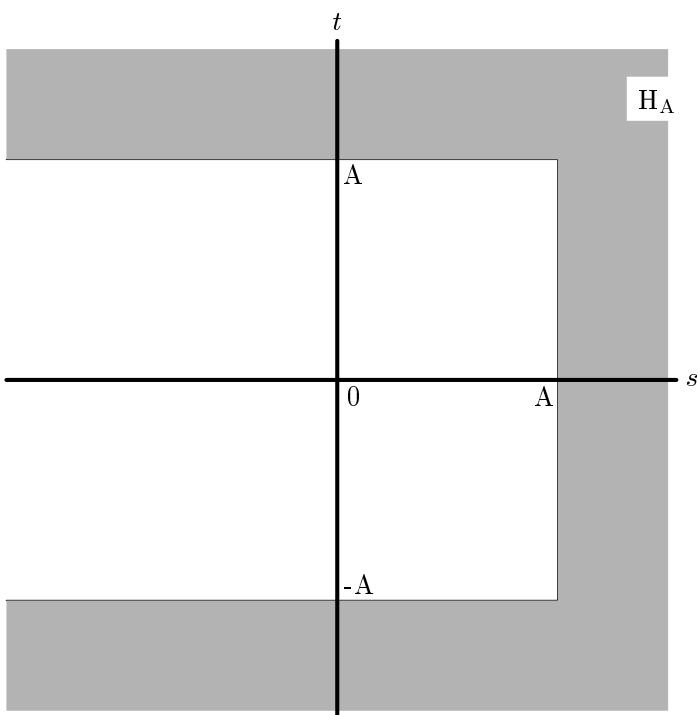
\includegraphics[keepaspectratio]{images/part002_194eed20.jpg}}\\
图 2

其中 \(C_{p}\) 仅依赖于 p。现设 F 是以诸集 \(H_{A}\) 为基的滤子；柯西准则表明，沿滤子 F ，函数 \(\log \Gamma(z) - g(z)\) 有一个有限极限 \(\delta\) （模 \(2\pi i\) ） ，并且，若令 \(\omega(z) = \max(\mathcal{R}(z), |\mathcal{I}(z)|)\) ，则有

\[
\log \Gamma (z) - g (z) - \delta \equiv O \left(\frac {1}{(\omega (z)) ^ {2 p}}\right) \pmod {2 \pi i}.\tag{18}
\]

对实数 \(x\) 且 \(> 0\) ，有 \(\Gamma(x) > 0\) ，且 \(g(x)\) 是实数，故可以设 \(\delta\) 是实数，并有

\[
\log \Gamma (x) = g (x) + \delta + O \left(\frac {1}{x ^ {2 p}}\right).
\]

现在来确定常数 \(\delta\) 的值；把 VII, p.~318 的 prop. 2 应用于 p = 2 ，则当实数 x 趋于 \(+\infty\) 时，有

\[
\begin{array}{c} \frac {x - 1}{2} \log \frac {x}{2} - \frac {x}{2} + \frac {x}{2} \log \frac {x + 1}{2} - \frac {x + 1}{2} + 2 \delta \\ = x \log x - x - \frac {1}{2} \log x + (\frac {1}{2} - x) \log 2 + \frac {1}{2} \log 2 \pi + \delta + o (1) \end{array}
\]

由此容易推出 \(\delta = \frac{1}{2}\log 2\pi\) 。最后有下列结果：

命题 4. 沿滤子 \(\mathfrak{F}\) ，有（对每个整数 \(p \geqslant 1\) ）渐近展开

\[
\begin{array}{l} \log \Gamma (z) \equiv z \log z - z - \frac {1}{2} \log z + \frac {1}{2} \log 2 \pi \\ \quad + \sum_ {k = 1} ^ {p} \frac {b _ {2 k}}{2 k (2 k - 1)} \frac {1}{z ^ {2 k - 1}} + O \left(\frac {1}{(\omega (z)) ^ {2 p}}\right) \pmod {2 \pi i} \end{array}\tag{19}
\]

（斯特林展开）。

推论. 沿滤子 F ，有

\[
\Gamma (z) \sim \sqrt {2 \pi} \exp (z \log z - z - \frac {1}{2} \log z).\tag{20}
\]

特别地，当实数 \(x\) 趋于 \(+\infty\) 时，公式 (20) 可以写成

\[
\Gamma (x) \sim \sqrt {2 \pi} x ^ {x - 1 / 2} e ^ {- x},\tag{21}
\]

于是，当整数 n 趋于 \(+\infty\) 时，

\[
n! \sim \sqrt {2 \pi} n ^ {n + 1 / 2} e ^ {- n}
\]

（cf.~V, p.~244）。

由此可以导出许多公式。例如，对每个复数 \(\alpha\) 与每个整数 n ，当 n 趋于 \(+\infty\) 时，有

\[
\frac {\Gamma (n + \alpha)}{\Gamma (n)} \sim n ^ {\alpha} \quad (= e ^ {\alpha \log n}).\tag{22}
\]

同样，对每个不是整数 \(\leqslant 0\) 的复数 a ，有

\[
a (a + 1) (a + 2) \dots (a + n) = \frac {\Gamma (n + a + 1)}{\Gamma (a)} \sim \frac {\sqrt {2 \pi}}{\Gamma (a)} n ^ {n + a + 1 / 2} e ^ {- n}\tag{23}
\]

而对每个不是整数 \(\geqslant 0\) 的复数 a ，有

\[
\binom {a} {n} = \frac {(- 1) ^ {n}}{\Gamma (- a)}   \frac {\Gamma (n - a)}{\Gamma (n + 1)} \sim \frac {(- 1) ^ {n}}{\Gamma (- a)}   n ^ {- a - 1}.\tag{24}
\]

最后，对每个实常数 \(k > 1\) ，有

\[
\binom {k n} {n} = \frac {\Gamma (k n + 1)}{\Gamma (n + 1)   \Gamma ((k - 1) n + 1)} \sim \sqrt {\frac {k}{2 \pi (k - 1) n}} \left(\frac {k ^ {k}}{(k - 1) ^ {k - 1}}\right) ^ {n}.\tag{25}
\]

同样的论证导出下面类似的命题：

命题 5. 沿滤子 \(\mathfrak{F}\) ，有（对每个整数 \(p \geqslant 1\) ）渐近展开

\[
\frac {\Gamma^ {\prime} (z)}{\Gamma (z)} = \log z - \frac {1}{2 z} - \sum_ {k = 1} ^ {p} \frac {b _ {2 k}}{2 k} \frac {1}{z ^ {2 k}} + O \left(\frac {1}{(\omega (z)) ^ {2 p + 1}}\right).\tag{26}
\]

这里不用 VII, p.~318 的 prop. 2 ，而使用公式

\[
\int_ {x} ^ {x + 1} \frac {\Gamma^ {\prime} (t)}{\Gamma (t)} d t = \log \Gamma (x + 1) - \log \Gamma (x) = \log x
\]

来确定常数。

\setcounter{exercisegroup}{0}
\refstepcounter{exercisegroup}
\section*{第 \S\arabic{exercisegroup} 节习题}
\phantomsection
\addcontentsline{toc}{section}{第 \protect\S\arabic{exercisegroup} 节习题}

J 1) 设 \(g\) 是一个规则函数，且 \(>0\) （在 \(]0, +\infty[\) 上）。

\begin{enumerate}
\def\labelenumi{\alph{enumi})}
\tightlist
\item
  设 \(u, v\) 是 \(]0, +\infty[\) 上的两个递增函数，使得 \(u(x + 1) - u(x) = v(x + 1) - v(x) = g(x)\) （对一切 \(x > 0\) ）。证明：若 \(w = u - v\) ，则
\end{enumerate}

\[
\sup _ {0 <   x \leqslant y \leqslant 1} | w (y) - w (x) | \leqslant \inf _ {x > 0} g (x).
\]

（注意，对 \(a \leqslant x \leqslant y \leqslant a + 1\) 有 \(u(y) - u(x) \leqslant g(a)\) 。）特别地，若 \(\inf_{x > 0} g(x) = 0\) ，则在一点处取给定值的方程 \(u(x + 1) - u(x) = g(x)\) 的递增解至多只有一个。

\begin{enumerate}
\def\labelenumi{\alph{enumi})}
\setcounter{enumi}{1}
\tightlist
\item
  设 g 在 {]}0, +∞{[} 上递减。证明级数
\end{enumerate}

\[
\varphi (x) = - g (x) + \sum_ {n = 1} ^ {\infty} (g (n) - g (x + n))
\]

在含于 {]}0, +∞{[} 的每个紧区间上绝对且一致收敛；若 \(\lambda = \lim_{x \to +\infty} g(x)\) ，则函数 \(u(x) = \varphi(x) + \lambda x\) 是方程 \(u(x+1) - u(x) = g(x)\) 的一个递增解。证明：对这个方程的每个递增解 v ，有 \(v(y) - v(x) \geqslant \varphi(y) - \varphi(x)\) （对 0 \textless{} x \textless{} y）。在一点处取给定值的方程 \(u(x+1) - u(x) = g(x)\) 的递增解所成的集，其上（相应地，下）包络是什么？证明这个集仅由一个元素组成当且仅当 \(\lambda = 0\) 。c) 证明：若 \(g(x)\) 递增且 \textgreater0 （在 {[}0, +∞{]} 上），则在一点处取给定值的方程 \(u(x+1) - u(x) = g(x)\) 有无穷多个递增解。d) 设 \(\psi(x)\) 是在 {]}0, +∞{[} 上由下列条件定义的函数：\(\psi(x)=0\) （对 \(0\leqslant x<1\) ）；\(\psi(x)=1\) （对 \(1\leqslant x<2\) ）；\(\psi(x)=n\) （对 \(n-1+\frac{1}{n-1}\leqslant x<n+\frac{1}{n}\) ， \(n\geqslant2\) ）；令 \(g(x)=\psi(x+1)-\psi(x)\) 。证明 \(\psi\) 是方程

\[
u (x + 1) - u (x) = g (x)
\]

使得 \(u(1)=1\) 的唯一递增解。

J2) 设 g 是 {]}0, +∞{[} 上的连续递增函数。

\begin{enumerate}
\def\labelenumi{\alph{enumi})}
\item
  证明：若 \(\liminf_{x\to +\infty}g(x) / x = 0\) ，则在一点处取给定值的方程 \(u(x + 1) - u(x) = g(x)\) 的凸解至多只有一个（注意，对一切 \(h > 0\) ，函数 \(v(x) = u(x + h) - u(x)\) 是满足方程 \(v(x + 1) - v(x) = g(x + h) - g(x)\) 的递增函数，并应用 exerc. 1 a））。
\item
  证明：若 g 在 \(]0, +\infty[\) 上是凹的，则方程 \(u(x+1) - u(x) = g(x)\) 存在凸解；这个方程在一点处取给定值的凸解存在且唯一，当且仅当 \(\lim_{x \to +\infty} g(x)/x = 0\) （cf.~exerc. 1 b））。
\item
  以下设 \(g\) 在 \(]0, +\infty[\) 上递增且凹，并且 \(\lim_{x \to +\infty} g(x) / x = 0\) 。对每对数 \(h > 0\) 、\(k > 0\) 以及每个有限实值函数 \(f\) （定义在 \(]0, +\infty[\) 上），令
\end{enumerate}

\[
\varDelta \Big (f (x); h, k \Big) = \frac {f (x + h) - f (x)}{h} - \frac {f (x) - f (x - k)}{k}
\]

对 x \textgreater{} k。证明：若 u 是方程 \(u(x + 1) - u(x) = g(x)\) 的一个凸解，则有 \(\lim_{x \to +\infty} \Delta(u(x); h, k) = 0\) （对一切 h \textgreater{} 0 与 k \textgreater{} 0）（利用 VII, p.~325 的 exerc. 1 b) 中 \(u_{r}^{\prime}\) 的表达式）。

\(d\) ）用 \(c\) ）的记号证明：存在常数 \(\alpha\) ，使得 \(u(x) = v(x) + \alpha\) ，其中

\[
v (x) = \int_ {1} ^ {x} g (t) d t - \frac {1}{2} g (x) + R (x)
\]

这里令

\[
\mathrm{R} (x) = \sum_ {n = 0} ^ {\infty} h (x + n), \quad h (x) = \int_ {x} ^ {x + 1} g (t) d t - \frac {1}{2} (g (x + 1) + g (x));
\]

并且有

\[
0 \leqslant \mathrm{R} (x) \leqslant \frac {1}{2} (g (x + \frac {1}{2}) - g (x)).
\]

（注意 \(v(x + 1) - v(x) = g(x)\) ，且 \(\lim_{x\to +\infty}\Delta (v(x);h,k) = 0\) （不论 \(h > 0\) 与 \(k > 0\) 如何）。）

\begin{enumerate}
\def\labelenumi{\arabic{enumi})}
\setcounter{enumi}{2}
\tightlist
\item
  \begin{enumerate}
  \def\labelenumii{\alph{enumii})}
  \tightlist
  \item
    设 g 是一个具有连续 \(k^{th}\) 导数的函数，定义在 {]}0, +∞{[} 上，\(g^{(k)}\) 在此区间上递减且 \(\lim_{x\to+\infty}g^{(k)}(x)=0\) 。证明：方程 \(u(x+1)-u(x)=g(x)\) 存在唯一的解 u ，它具有递增的 \(k^{th}\) 导数（在 {]}0, +∞{[} 上）且在一点取给定值（利用 exerc. 1 b)）。
  \end{enumerate}
\end{enumerate}

\begin{enumerate}
\def\labelenumi{\alph{enumi})}
\setcounter{enumi}{1}
\tightlist
\item
  设 \(\alpha\) 是任意实数。设 \(S_{\alpha}\) 是定义在 \(]0, +\infty[\) 上、满足关系式
\end{enumerate}

\[
\mathrm{S} _ {\alpha} (x + 1) - \mathrm{S} _ {\alpha} (x) = x ^ {\alpha}
\]

使 \(S_{\alpha}(1) = 0\) ，此外，\(S_{\alpha}\) 的以 \((\alpha + 1)^{+}\) 的整数部分为阶的导数是递增的（由 \(a\) )，它是唯一的函数）。证明

\[
\mathrm{S} _ {\alpha} ^ {\prime} (x) - \mathrm{S} _ {\alpha} ^ {\prime} (1) = \alpha \mathrm{S} _ {\alpha - 1} (x),
\]

以及

\[
\mathrm{S} _ {\alpha} \left(\frac {x}{p}\right) + \mathrm{S} _ {\alpha} \left(\frac {x + 1}{p}\right) + \dots + \mathrm{S} _ {\alpha} \left(\frac {x + p - 1}{p}\right) = \frac {1}{p ^ {\alpha}} \mathrm{S} _ {\alpha} (x) + \mathrm{C} _ {\alpha}
\]

对每个整数 \(p \geqslant 1\) 成立，其中 \(C_{\alpha}\) 是常数，当 \(\alpha \neq -1\) 时它等于

\[
\left(\frac {1}{p ^ {\alpha}} - p\right) \frac {S _ {\alpha + 1} ^ {\prime} (1)}{\alpha + 1}
\]

（cf.~VII, p.318, prop. 2 与 VI, p.~291, exerc. 3）。

\begin{enumerate}
\def\labelenumi{\arabic{enumi})}
\setcounter{enumi}{3}
\tightlist
\item
  证明函数 \(f(x) = \frac{1}{\sqrt{2}}\frac{\Gamma(x / 2)}{\Gamma\left(\frac{x + 1}{2}\right)}\) 是方程
\end{enumerate}

\(u(x + 1) = 1 / x \, u(x)\) 的唯一凸解（注意此方程蕴含 \(u(x + 2) = \frac{x}{x + 1} \, u(x)\) ，并应用 exerc. 1 a））。

\begin{enumerate}
\def\labelenumi{\arabic{enumi})}
\setcounter{enumi}{4}
\item
  把 VII, p.~310 与 311 的引理 1 与引理 2 推广到任意的对数凸函数（cf.~I, p.~45, exerc. 2）。证明每个对数凸函数都是凸的。
\item
  设 \(\psi(x) = \Gamma'(x)/\Gamma(x)\) ；对每个整数 \(q > 1\) 与每个整数 \(k\) （使 \(1 \leqslant k \leqslant q - 1\) ），建立公式
\end{enumerate}

\[
\sum_ {p = 1} ^ {q} \psi \left(\frac {p}{q}\right) \exp \left(\frac {2 p k \pi i}{q}\right) = - q \sum_ {n = 1} ^ {\infty} \frac {1}{n} \exp \left(\frac {2 n k \pi i}{q}\right) = q \log \left(1 - \exp \frac {2 k \pi i}{q}\right).
\]

（利用 VII, p.~307 的公式 (9)。）

\setcounter{exercisegroup}{1}
\refstepcounter{exercisegroup}
\section*{第 \S\arabic{exercisegroup} 节习题}
\phantomsection
\addcontentsline{toc}{section}{第 \protect\S\arabic{exercisegroup} 节习题}

\(\mathfrak{J}1)\) a) 设 \(g\) 是 \(x \geqslant 0\) 上的连续实值函数。证明：若 \(g\) 满足两个恒等式

\[
\sum_ {k = 0} ^ {p - 1} g \left(\frac {x + k}{p}\right) = g (x)
\]

\[
\sum_ {h = 0} ^ {q - 1} g \left(\frac {x + h}{q}\right) = g (x)
\]

则它也满足恒等式

\[
\sum_ {j = 0} ^ {p q - 1} g \left(\frac {x + j}{p q}\right) = g (x).
\]

\begin{enumerate}
\def\labelenumi{\alph{enumi})}
\setcounter{enumi}{1}
\tightlist
\item
  由此推出：若函数 \(g\) 在 \(x \geqslant 0\) 上有连续导数且满足恒等式
\end{enumerate}

\[
\sum_ {k = 0} ^ {p - 1} g \left(\frac {x + k}{p}\right) = g (x)
\]

则它具有 \(a(x-\frac{1}{2})\) 的形式，其中 a 是常数（注意 g 满足把 p 换成 \(p^{n}\) 后的类似恒等式；令 n 趋于 \(+\infty\) ，推出 \(g'(x)=\int_{0}^{1}g'(t)dt\) ）。c) 由 b) 断定：\(\Gamma\) 函数是在 x\textgreater0 上有连续导数、且对 p 的某个值满足 VII, p.~305 的方程 (1) 与 VII, p.~318 的倍乘公式 (12) 的唯一函数。

\begin{enumerate}
\def\labelenumi{\arabic{enumi})}
\setcounter{enumi}{1}
\tightlist
\item
  对每个整数 \(k > 1\) ，令 \(S_k = \sum_{n=1}^{\infty} n^{-k}\) 。证明：对 \(-1 < x \leqslant 1\) ，有
\end{enumerate}

\[
\log \Gamma (1 + x) = - \gamma x + \sum_ {k = 2} ^ {\infty} (- 1) ^ {k} \frac {\mathrm{S} _ {k}}{k} x ^ {k}
\]

右端的级数在 \(]-1,1]\) 的每个紧子集上一致收敛，且对 \(|x|<1\) 绝对收敛。

\begin{enumerate}
\def\labelenumi{\arabic{enumi})}
\setcounter{enumi}{2}
\tightlist
\item
  设 s 是固定的实数；证明：当 t 趋于 \(+\infty\) 或 \(-\infty\) 时，有
\end{enumerate}

\[
| \Gamma (s + i t) | \sim \sqrt {2 \pi} | t | ^ {s - 1 / 2} e ^ {- (\pi / 2) | t |}
\]

以及

\[
\frac {\Gamma^ {\prime} (s + i t)}{\Gamma (s + i t)} \sim \log | t |.
\]

\begin{enumerate}
\def\labelenumi{\arabic{enumi})}
\setcounter{enumi}{3}
\tightlist
\item
  设 t 是固定的实数 \(\neq 0\) ；证明：当 s 趋于 \(+\infty\) 时，
\end{enumerate}

\[
| \Gamma (- s + i t) | \sim \sqrt {\frac {\pi}{2}} \left(s ^ {s + 1 / 2} e ^ {- s} \sqrt {\sinh^ {2} \pi t + \sin^ {2} \pi s}\right) ^ {- 1}
\]

（利用余元公式）。

\begin{enumerate}
\def\labelenumi{\arabic{enumi})}
\setcounter{enumi}{4}
\tightlist
\item
  设 \(x_{n}\) 是方程 \(\Gamma'(x) = 0\) 在区间 \(] - n, -n + 1[\) 中的根。证明
\end{enumerate}

\[
x _ {n} = - n + \frac {1}{\log n} + O \left(\frac {1}{(\log n) ^ {2}}\right)
\]

（利用余元公式与 VII, p.~316 的公式 (5)）。由此推出

\[
\Gamma (x _ {n}) \sim \frac {(- 1) ^ {n}}{\sqrt {2 \pi}} n ^ {- n - 1 / 2} e ^ {n + 1} \log n.
\]

\begin{enumerate}
\def\labelenumi{\arabic{enumi})}
\setcounter{enumi}{5}
\tightlist
\item
  设 \(V_{n}\) 是范德蒙德行列式 \(\mathrm{V}(1,2,\dots,n)\) （Alg., III, p.~532）。证明
\end{enumerate}

\[
\log V _ {n} = \frac {n ^ {2}}{2} \log n - \frac {3 n ^ {2}}{4} + \left(\frac {1}{2} \log 2 \pi - \frac {1}{4}\right) n - \frac {1}{12} \log n + k + O \left(\frac {1}{n}\right)
\]

其中 k 是常数。

\section*{历史注记}
\phantomsection
\addcontentsline{toc}{section}{历史注记}

（注意：罗马数字指本注记末尾的参考文献。）

对序列 \((u_{n})\) 用一个依赖于实参数 \(\lambda\) 且等于 \(u_{n}\) （当 \(\lambda = n\) 时）的积分的值进行``插值''的想法，可追溯到沃利斯（III, p.~55）。正是这一想法主要引导了欧拉，他在 1730 年（(I), v. XIV, p.~1-24）着手对阶乘序列进行插值。他首先注意到，\(n!\) 等于无穷乘积 \(\prod_{k=1}^{\infty}\left(\frac{k+1}{k}\right)^{n}\frac{k}{k+n}\) ，这个乘积对 n 的每个值（整数或非整数）都有定义，并且特别地，当 \(n = \frac{1}{2}\) 时由沃利斯公式可知它取值 \(\frac{1}{2}\sqrt{\pi}\) 。这一结果与沃利斯的结果之间的类比，促使他重新考察积分

\[
\int_ {0} ^ {1} x ^ {e} (1 - x) ^ {n} d x
\]

（n 为整数，e 任意），沃利斯已经考虑过它。欧拉利用二项展开得到它的值 \(\frac{n!}{(e+1)(e+2)\ldots(e+n+1)}\) ；一个变量替换又向他表明，\(n!\) 是积分 \(\int_{0}^{1}\left(\frac{1-x^{z}}{z}\right)^{n}dx\) 当 z 趋于 0 时的极限，由此得到``第二类欧拉积分''

\[
n! = \int_ {0} ^ {1} \left(\log \frac {1}{x}\right) ^ {n} d x;
\]

用同样的方法，并利用沃利斯公式，他得到公式 \(\int_0^1\sqrt{\log 1 / x} dx = \frac{1}{2}\sqrt{\pi}\) 。在他的后期著作中，欧拉经常回到这些积分；他就这样发现了余元公式（(I), t. XV, p.~82 与 t. XVII, p.~342）、公式 \(\mathbf{B}(p,q) = \Gamma (p)\Gamma (q) / \Gamma (p + q)\) （(I), t. XVII, p.~355）以及勒让德–高斯公式对应于 \(x = 1\) 的特殊情形（(I), t. XIX, p.~483）；所有这些当然都没有考虑收敛性问题。

高斯在关于超几何函数的研究中继续研究 \(\Gamma\) 函数，\(\Gamma\) 函数是超几何函数的一个极限情形（II）；正是在这项研究过程中他得到了一般的倍乘公式（勒让德稍早已对 p = 2 记下了它）。关于 \(\Gamma\) 的后期工作主要涉及把这个函数延拓到复数域。直到最近人们才认识到，对数凸这一性质在实数域上把 \(\Gamma(x)\) （相差一个常数因子）从泛函方程 \(f(x + 1) = x f(x)\) 的解中刻画出来（III）；阿廷（IV）指出了如何把 \(\Gamma(x)\) 的所有经典结果都简单地与这一性质联系起来。我们相当紧密地遵循了他的阐述。

\section*{参考文献}
\phantomsection
\addcontentsline{toc}{section}{参考文献}

\begin{enumerate}
\def\labelenumi{(\Roman{enumi})}
\item
L. EULER, Opera omnia, Leipzig-Berlin (Teubner): t. XIV (1924), t. XV (1927), t. XVII (1915) 与 t. XIX (1932).
\item
  C.F. GAUSS, Werke, t. III, Göttingen, 1866.
\item
  H. BOHR und J. MOLLERUP, Laerebog i matematisk Analyse, t. III, Kopenhagen, 1922, p.~149-164.
\item
  E. ARTIN, Einführung in die Theorie der Gammafunktion, Leipzig (Teubner), 1931.
\end{enumerate}

\backmatter
\chapter*{记号索引}
\phantomsection
\addcontentsline{toc}{chapter}{记号索引}

\begin{Shaded}
\begin{Highlighting}[]
\FunctionTok{Df(x0)}\KeywordTok{:}\AttributeTok{ }\DecValTok{5}
\FunctionTok{f\textquotesingle{}(x0)}\KeywordTok{:}\AttributeTok{ }\DecValTok{5}
\FunctionTok{f\textquotesingle{}d(x0)}\KeywordTok{:}\AttributeTok{ }\DecValTok{6}
\FunctionTok{f\textquotesingle{}g(x0)}\KeywordTok{:}\AttributeTok{ }\DecValTok{6}
\FunctionTok{Df}\KeywordTok{:}\AttributeTok{ }\DecValTok{7}
\FunctionTok{df/dx}\KeywordTok{:}\AttributeTok{ }\DecValTok{7}
\FunctionTok{f\textquotesingle{}d}\KeywordTok{:}\AttributeTok{ }\DecValTok{7}
\FunctionTok{f\textquotesingle{}g}\KeywordTok{:}\AttributeTok{ }\DecValTok{7}
\FunctionTok{D\^{}n f}\KeywordTok{:}\AttributeTok{ }\DecValTok{23}
\FunctionTok{f(n)}\KeywordTok{:}\AttributeTok{ }\DecValTok{23}
\FunctionTok{∫x0 f}\KeywordTok{:}\AttributeTok{ }\DecValTok{61}
\FunctionTok{∫x0 f(t) dt}\KeywordTok{:}\AttributeTok{ }\DecValTok{61}
\FunctionTok{∫x0\^{}x f}\KeywordTok{:}\AttributeTok{ }\DecValTok{61}
\FunctionTok{∫x0\^{}x f(t) dt}\KeywordTok{:}\AttributeTok{ }\DecValTok{61}
\FunctionTok{h(t)|x|\_\{x0\}}\KeywordTok{:}\AttributeTok{ }\DecValTok{62}
\FunctionTok{∫a(n) f}\KeywordTok{:}\AttributeTok{ }\DecValTok{66}
\FunctionTok{∫I f(t) dt}\KeywordTok{:}\AttributeTok{ }\DecValTok{69}
\FunctionTok{e}\KeywordTok{:}\AttributeTok{ }\DecValTok{97}
\FunctionTok{exp x}\KeywordTok{:}\AttributeTok{ }\DecValTok{97}
\FunctionTok{log x (x real \textgreater{} 0)}\KeywordTok{:}\AttributeTok{ }\DecValTok{97}
\FunctionTok{π}\KeywordTok{:}\AttributeTok{ }\DecValTok{99}
\FunctionTok{Arc cos x}\KeywordTok{:}\AttributeTok{ }\DecValTok{100}
\FunctionTok{Arc sin x}\KeywordTok{:}\AttributeTok{ }\DecValTok{100}
\FunctionTok{Arc tan x}\KeywordTok{:}\AttributeTok{ }\DecValTok{100}
\FunctionTok{cos x}\KeywordTok{:}\AttributeTok{ }\DecValTok{100}
\FunctionTok{cot x}\KeywordTok{:}\AttributeTok{ }\DecValTok{100}
\FunctionTok{csc x}\KeywordTok{:}\AttributeTok{ }\DecValTok{100}
\FunctionTok{sec x}\KeywordTok{:}\AttributeTok{ }\DecValTok{100}
\FunctionTok{sin x}\KeywordTok{:}\AttributeTok{ }\DecValTok{100}
\FunctionTok{tan x}\KeywordTok{:}\AttributeTok{ }\DecValTok{100}
\FunctionTok{e\^{}z}\KeywordTok{:}\AttributeTok{ }\DecValTok{103}
\FunctionTok{exp z}\KeywordTok{:}\AttributeTok{ }\DecValTok{103}
\FunctionTok{cos z}\KeywordTok{:}\AttributeTok{ }\DecValTok{107}
\end{Highlighting}
\end{Shaded}

cot z: 107 log z: 105 sin z: 107 tan z: 107 cosh x: 108 sinh x: 108 tanh x: 108 Arg cosh x: 109 Arg sinh x: 109 Arg tanh: 110 \(\binom{m}{n}\) : 114 \(e^{A}\) : 198 exp A: 198 \(\mathcal{H}(\mathfrak{F}, V)\) : 221 \(R_{\infty}\) : 221 \(\mathcal{H}_{\infty}(\mathfrak{F}, V)\) : 222 \(f_{1} \preccurlyeq f_{2}\) : 223 \(f_{2} \succcurlyeq f_{1}\) : 223 \(f \preccurlyeq g\) : 223 \(g \succcurlyeq f\) : 223 \(f + g\) : 223 fg: 223 fλ: 223 \textbar\textbar f\textbar\textbar: 223 f ≃ g: 224 \(f_{1} \prec f_{2}\) : 225 \(f_{2} \succcurlyeq f_{1}\) : 225 \(f \prec g\) : 225 \(g \succcurlyeq f\) : 225 f \textasciitilde{} g: 226 \(O(f), O_{k}(f), o(f), o_{k}(f)\) : 230 \(l_{0}(x), l_{n}(x)\) : 240 \(\mathfrak{K}(y) (\mathfrak{K} \text{ 一个 Hardy 域})\) : 261 \(e_{0}(x), e_{n}(x)\) : 265 \(\sum_{k=0}^{\infty} \alpha_{k} D^{k}\) : 285 \(B_{n}(X)\) : 288 \(b_{n}\) : 288 \(U_{x}^{\xi}(f(\xi))\) : 290 \(\Gamma(n), \Gamma(x)\) : 317 B (x, y): 324 \(\Gamma(z)\) : 327

\chapter*{索引}
\phantomsection
\addcontentsline{toc}{chapter}{索引}

\par\noindent\textbf{\texorpdfstring{wlog\textbackslash indfile=\textbackslash read1}{wlog=}}\par

添加（多项式的根、原函数、原函数的指数式）到微分域, 121

线性微分方程的伴随（方程）, 186

阿佩尔多项式, 272

微分方程的精确到 \(\varepsilon\) 的近似解, 166

渐近展开

- 比另一个更精确的, 222

- 函数相对于比较尺度的, 222

- 函数精确到 \(g_{\alpha}\) 的, 222

- 的精确度, 222

渐近展开, 220

- 变系数, 226

\par\noindent\textbf{伯努利数, 276}\par

伯努利多项式, 275

二项式公式, 108

二项级数, 109

卡莱曼不等式, 117

卡尔森不等式, 116

积分的柯西准则, 65

变量替换公式, 60

特征

- 局部, 211

系数

- 二项式, 21

比较尺度, 220

余元公式, 316

复合算子, 270

- 指示函数, 278

- 的阶, 272

- 正则, 279

余割, 95

余弦

- 双曲, 102

复数的余弦, 102

余切, 95

判别法

- 收敛

-- 第二类, 244

- 积分

-- 对数, 229

判别法

- 积分的柯西准则, 65

-- 柯西–麦克劳林, 237

- 叶尔马科夫, 86

\par\noindent\textbf{达朗贝尔}\par

-- 收敛判别法, 245

(H) 函数的定义序列, 252

导数

- 一阶, 3

- 无穷, 10

- 对数, 94

- \(n^{th}\) , 20

- 二阶, 20

- 对称, 39

函数的导数, 3

- 左, 4

- 右, 4

由 \(n\) 个线性微分方程构成的方程组的 \(n\) 个积分（解）的行列式, 184

微分方程

- 伴随, 187

- 积分, 163

- 线性, 177

- 线性齐次, 178

- \(n\) 阶线性, 192

- 利普希茨, 171

- 局部利普希茨, 171

- 一阶, 164

- \(n\) 阶, 164

-- 实变量, 163

- 数量, 164

- 解, 163

\par\noindent\textbf{336}\par

\par\noindent\textbf{索引}\par

\par\noindent\textbf{域}\par

域 - 微分, 121 公式 - 变量替换, 60 - 欧拉–麦克劳林求和, 282 - 高斯, 307 - 分部积分, 60 - n 阶分部积分, 60 - 勒让德–高斯倍乘, 318 - 莱布尼茨, 20 - 斯特林, 243 - 泰勒, 21 - 沃利斯, 123 - 魏尔斯特拉斯, 308 公式 - 欧拉, 99 函数 - n 次可导 -- 在一点, 20 -- 在区间上, 20 - (H), 252 - 凹, 26 - 凸, 26 - 导函数, 4 - 可导 -- 在一点, 3 -- 无穷次, 20 -- 在区间上, 4 - 一函数受另一函数控制, 212 - 初等, 122

函数的广义泰勒展开, 278

多项式的广义泰勒展开, 274

与复合算子相联系的阿佩尔多项式的生成级数, 275

阿达马不等式, 118

哈代–李特尔伍德不等式, 89

哈代–李特尔伍德陶伯定理, 45

埃尔米特多项式, 282

赫拉夫卡不等式, 90

双曲函数, 102

赫尔德不等式, 115

\par\noindent\textbf{恒等式}\par

- 雷德赫费尔, 88

无穷次可导函数, 20

复合算子的指示函数, 278 不等式

- 卡莱曼, 117

- 卡尔森, 116

-- 柯西–布尼亚科夫斯基–施瓦茨, 115

- 柯西–施瓦茨, 88

- 阿达马, 118

- 哈代, 117

- 哈代–李特尔伍德, 89

- 赫拉夫卡, 90

- 赫尔德, 115

- 奥皮亚尔, 90

- 外尔, 90

积分

- 绝对收敛, 67

- 收敛, 63

- 欧拉, 310

- 高斯, 314

- 正规收敛, 71, 73

- 分段规则函数的, 63

- 规则函数在

非紧区间上的, 63

- 微分方程的, 163

- 拉阿贝, 318

- 一致收敛, 71

分部积分公式, 60

\(n\) 阶分部积分公式, 60

迭指数, 253

迭对数, 229

\par\noindent\textbf{库默尔同余（式）, 295}\par

\par\noindent\textbf{莱布尼茨公式, 20}\par

直线

- 局部在图像上方, 31

- 局部在图像下方, 31

- 局部位于图像上, 31

刘维尔定理, 122

利普希茨条件, 168

利普希茨微分方程, 171

利普希茨函数, 171

局部性, 211

对数

- 迭, 229

- 纳皮尔, 92

- 自然, 92

极大

- 复数的, 100

- 主值, 100

对数导数, 94

对数有界函数, 214

对数凸函数, 310

- 相对, 11

-- 严格, 11

\par\noindent\textbf{平均}\par

- 算术, 93

-- 加权, 93

- 几何, 93

-- 加权, 93

函数的平均值, 58

中值定理, 14

常数变易法, 182

极小

- 相对, 11

-- 严格, 11

纳皮尔对数, 92

自然对数, 92

牛顿多边形, 259

正规收敛积分, 71

\par\noindent\textbf{算子}\par

- 复合, 270

- 平移, 270

奥皮亚尔不等式, 90

一函数相对于另一函数的阶, 218

佩亚诺定理, 167

分段规则函数, 63

多边形

- 牛顿, 259

多项式

- 阿佩尔, 272

- 伯努利, 275

- 埃尔米特, 282

占优

- 一函数对另一函数, 214

素数

- 非正则, 295

- 正则, 295

原函数

- 函数在 \(\mathbf{R}\) 的区间上的, 51

- \(n\) 阶, 62

- 二阶, 62

- 严格, 51

主部

- 函数相对于比较尺度的, 221

- 函数相对于比较尺度与系数域的, 227

积分比较原理, 66

\par\noindent\textbf{索引}\par

拉阿贝积分, 318

拉阿贝判别法, 244

雷德赫费尔恒等式, 88

精确到 \(g_{\alpha}\) 的

- 函数的渐近展开, 222

正则复合算子, 279

规则函数, 54

\par\noindent\textbf{余项}\par

- 渐近展开中的, 222

-- 欧拉–麦克劳林公式中的, 283

- 泰勒公式中的, 22

线性微分方程的预解式, 180

罗尔定理, 12

根

- 常系数线性微分方程的特征根, 190

比较尺度, 220

正割, 95

第二中值定理, 82

相似函数, 214

正弦

- 双曲, 102

复数的正弦, 102

微分方程的精确到 \(\varepsilon\) 的解, 166

斯特林公式, 243

严格原函数, 51

微分方程的严格解, 164

严格

- 在图像上方, 23

- 在图像下方, 23

严格凹函数, 26

严格凸函数, 25

凸函数图像的支撑直线, 29

方程组

微分方程组, 164 - 数量微分方程的线性方程组的基本积分组, 183

\par\noindent\textbf{切线}\par

- 半

-- 左, 11

-- 右, 11

- 双曲, 102

- 图像的, 11

泰勒展开, 22

泰勒公式, 21

- \(n\) 阶, 22

\par\noindent\textbf{判别法}\par

- 达朗贝尔, 245

- 拉阿贝, 244

\par\noindent\textbf{定理}\par

- 柯西存在定理, 171

-- 克劳森–冯·施陶特, 294

-- 哈代–李特尔伍德陶伯, 45

- 刘维尔, 122

- 中值, 14

- 佩亚诺, 167

- 罗尔, 12

定理

- 杜·布瓦–雷蒙, 265

平移算子, 270

\par\noindent\textbf{一致收敛积分, 71}\par

\par\noindent\textbf{值}\par

- 函数的平均值, 58

常数变易

- 法, 182

沃利斯公式, 123

魏尔斯特拉斯公式, 308

外尔不等式, 90

\(n\) 阶线性微分方程的 \(n\) 个积分（解）的朗斯基行列式, 193
